\documentclass[conference]{IEEEtran}

\usepackage{amsmath}   % For advanced math symbols
\usepackage{graphicx}  % For including images
\usepackage{cite}      % For handling citations
\usepackage[hidelinks=true]{hyperref}  % For hyperlinks
\usepackage{lipsum}    % For example/filler text

% All separate paragraphs in italics in the document below act as commentary to explain where content came from or stuff that still needs to be done. This MUST be all deleted before submission

% *** TITLE AND AUTHOR ***
\title{Electronically Switching TIA Design \\
    \large ENGR302 Final Project Report - 2024}

\author{
    \IEEEauthorblockN{Evgeny Zhilkin, Louis Smith, Mario Pankusz, Max Mawby}
    \IEEEauthorblockA{
        Electrical \& Electronics Engineering \\
        Te Herenga Waka - Victoria University of Wellington \\
        Wellington, Aotearoa New Zealand \\
    }
}

\begin{document}

\maketitle

% *** ABSTRACT ***
\begin{abstract}

The Measurement Standards Laboratory of New Zealand (MSL) need a transimpedence amplifier whose gain can be switched remotely, to streamline the process of measuring low level currents from photodiodes. This project aimed to solve their problem by building a TIA with electronic switches that are controlled by a microcontroller to select gain, via an ethernet cable.\\

\end{abstract}


% *** INTRODUCTION ***
\section{Introduction}

\textit{Still needs: a summary of the evaluation section, basically the outcome or "findings" of the project.} \\

The New Zealand Measurement Standards Laboratory (NZMSL) plays a crucial role in ensuring the accuracy of measurement standards in New Zealand. One of their key responsibilities is the precise measurement of light levels from different sources, which is fundamental for applications ranging from environmental monitoring to industrial quality control. Accurate light measurement is vital for maintaining consistency in standards and ensuring that industries can rely on these measurements for their processes. In order to maintain accuracy, anytime the testing room is exposed to light there is down time to ensure light levels return to the baseline. NZMSL would like to reduce this down time, by reducing the number of times a person has to physically enter the room during a testing session. The goal of this project was to design a system that can be controlled remotely to solve this issue. \\

The current setup at NZMSL involves manual gain control on their transimpedence amplifier (TIA) that they use to measure small photodiode currents. Manually switching gain requires entering the experiment room , resulting in a loss of time as the room must darken again. This project involves designing a solution that enables remote gain switching without exposing the experiment to light, significantly reducing the downtime and allowing gain adjustments without interrupting the experimental environment.
Since NZMSL conducts experiments across a wide range of photodiodes, the solution must perform effectively within an operating current range from nano amps (nA) to milliamps (mA). Given NZMSL's role as a standard for measurements, it is crucial to ensure the solution's accuracy. This requires minimising interference with the input signal and carefully selecting components to reduce noise and inaccuracies in the amplification and switching circuits. \\

The remainder of this report will delve into: documented examples of TIA designs that were used to inform the outcomes of this project, the design and its various parts, implementation of the design, evaluation of the final design, final remarks and what could be done in the future to improve the design.

% *** MAIN BODY ***
\section{Related Work}

\textit{This section should provide a comprehensive overview of existing research and literature relevant to the topic, demonstrating your understanding of the field.} \\

Texas Instruments have published an in-depth exploration of designing transimpedance amplifiers (TIAs) for applications requiring the amplification of extremely low currents (such as nA) [1]. The TIA is crucial in converting this tiny input current into a corresponding output voltage, making it suitable for this application which demands precise current measurement and control. To achieve a 0-10V output range, the amplifier design must carefully consider the feedback resistor, as its value directly determines the voltage output for a given input current. For an input current of nanoamps, the feedback resistor would need to be in the range of M$\Omega$. Additionally, selecting an operational amplifier with ultra-low input bias current and low noise characteristics is essential to maintain signal integrity and accuracy at such low current levels. The document emphasises the importance of ensuring stability and managing bandwidth limitations, which are critical when dealing with high gain configurations in TIA circuits.

Another document from Texas Instruments [2] gives a detailed guide on designing a photodiode amplifier using an operational amplifier configured as a trans-impedance amplifier. It is designed to amplify a light-dependent current from a photodiode resulting in an analogue voltage output. The document outlines key design considerations, such as selecting the appropriate gain resistor and feedback capacitor to meet desired bandwidth requirements which in this case is 0. The circuit is specifically designed with a 5V supply voltage, aiming to achieve a maximum output voltage of 4.9V with a minimum input current of 0A which in this application will need to be modified to allow for the 0V – 10V range required on the output. The design process is supported by detailed simulations and recommended component choices, particularly the OPA323 op amp, known for its low bias current and rail-to-rail output capabilities which may be required if using ground as the negative rail in this amplifier. This document serves as a comprehensive reference for designing photodiode amplifier circuits with robust performance in various applications.

An article [3] by Black and Brisebois (Linear Technology) provides another view of an in-depth analysis of the requirements and challenges in designing transimpedance amplifiers for wide-range photodiodes, particularly in high-speed and high dynamic range applications. It discusses the critical role of low input bias current, low noise, and low input capacitance in achieving optimal TIA performance. The authors emphasise the importance of selecting amplifiers with FET input stages to minimise input current variation with temperature, as well as the need for careful board layout to reduce stray capacitances and leakage currents. Additionally, the consideration of adding a feedback capacitor is highlighted as a crucial step for ensuring circuit stability by compensating for input capacitance. The LTC6268 op amp is highlighted as a solution that meets these stringent requirements, offering femtoampere-level input bias current, high bandwidth, and low noise, making it ideal for advanced photodiode circuits. The discussion also underscores the trade-offs between gain, noise, and bandwidth in TIA design, illustrating the complexity of achieving stability and precision in such circuits.

In another article [4], Bonnie Baker delves into the task of designing transimpedance amplifiers for precision photo-sensing applications. Baker emphasises the importance of achieving the correct phase margin, which is required for determining the circuit’s step response, overshoot characteristics, and quality factor. The article outlines a systematic approach to TIA design, beginning with defining the operational amplifier's output swing and progressing to the calculation of the feedback resistor and capacitor, which are central to setting the desired phase margin. A detailed discussion on the calculation of key frequencies and the impact of feedback components on circuit stability and bandwidth highlights the delicate balance needed in TIA design. Additionally, Baker underscores the importance of selecting an amplifier with low input bias current and offset voltage, as well as the iterative process of fine-tuning the feedback capacitor to achieve a preferred phase margin. The article also considers the role of parasitic capacitances and the necessity of incorporating a feedback capacitor within the design to ensure stability. Through a practical example involving the Texas Instruments OPA192IDBVR and Vishay's TEMD6200FX01 photodiode, Baker illustrates the application of these design principles, providing engineers with valuable insights into the optimization of TIA circuits for precision opto-sensing.\\

The primary takeaway from these previous works is the importance in the specific op-amp selection. In particular for our purposes, a low input bias current and offset voltage are the most important factors. Because the input from NZMSL's photodiode will essentially be a DC current, there is little reason to be concerned with frequency response characteristic like bandwidth for this project. 

\textit{Copied from progress report, edited, still need to setup the references in this doc}

\section{Design}

\textit{The aim of this section is to articulate the technical solution with sufficient detail and clarity. When solving a complex problem, there are normally many different approaches one can take — each with its own advantages and disadvantages. It is expected that groups will initially consider a range of different solutions and narrow these down. The reasons why a particular approach was discounted should be documented here.} \\

At the most basic level there are three components or parts to the design. A microprocessor, switching circuit, and the transimpedance amplifier (TIA) circuit(s). Figure \ref{fig:1} illustrates the following process: a microprocessor controls the switching circuit which directs the path of the input current (from the client’s photodiode) through the TIA. This effectively gives the microcontroller the ability to set the gain of the system. \\

Figure \ref{fig:2} provides an alternative illustration of the fundamental workings of the design, including the basic arrangement of a TIA circuit. By changing the value of the feedback resistor between values on the order of $10^3$ to $10^9$, the TIA can output any current between 1nA to 1mA as a 1-10V voltage, satisfying requirements 1.1 and 2.1.

\begin{figure}
    \centering
    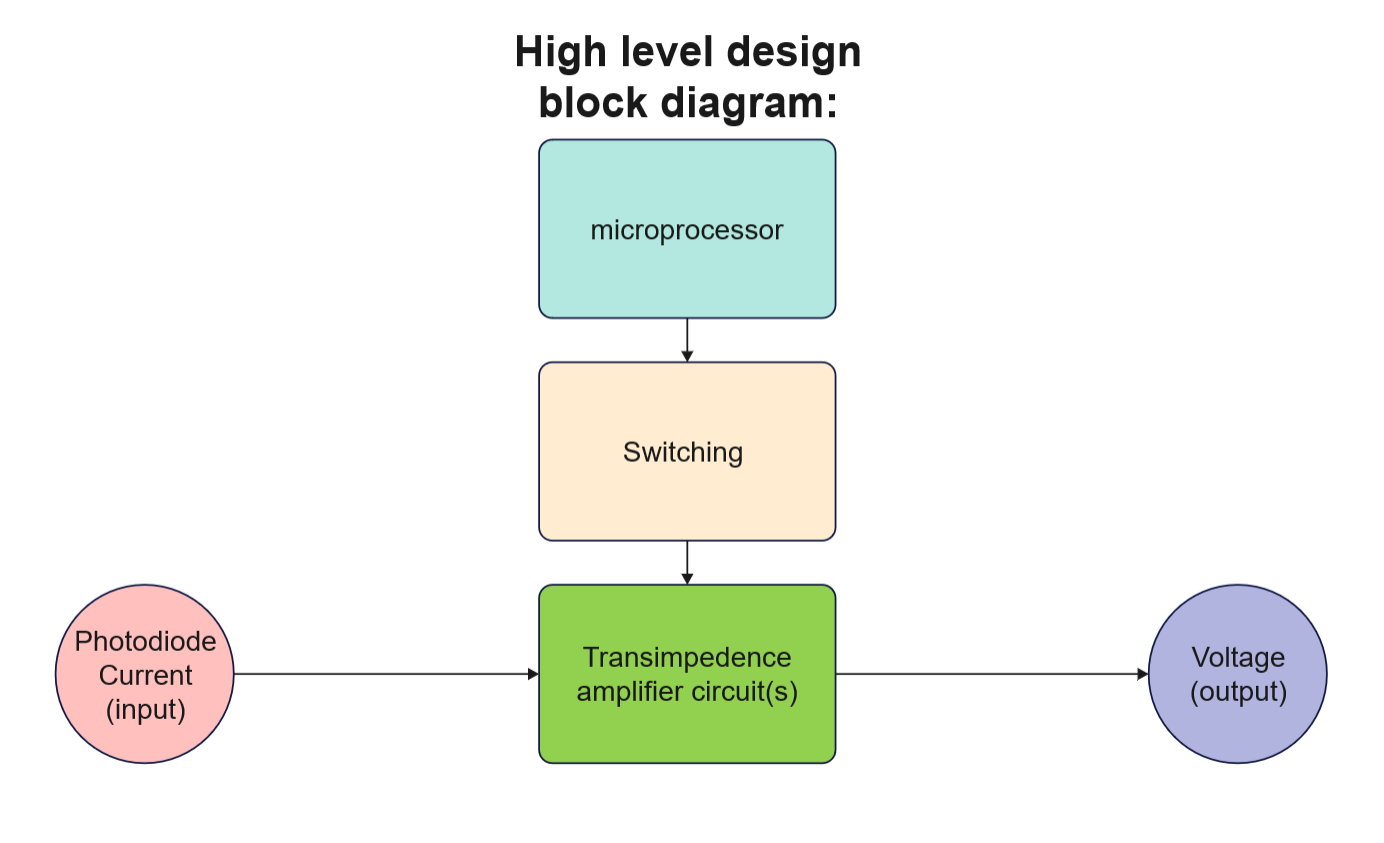
\includegraphics[width=0.8\linewidth]{ENGR302_TIA_blockl_diagram_v2.png}
    \caption{High level block diagram of the switching TIA design.}
    \label{fig:1}
\end{figure}

\begin{figure}
    \centering
    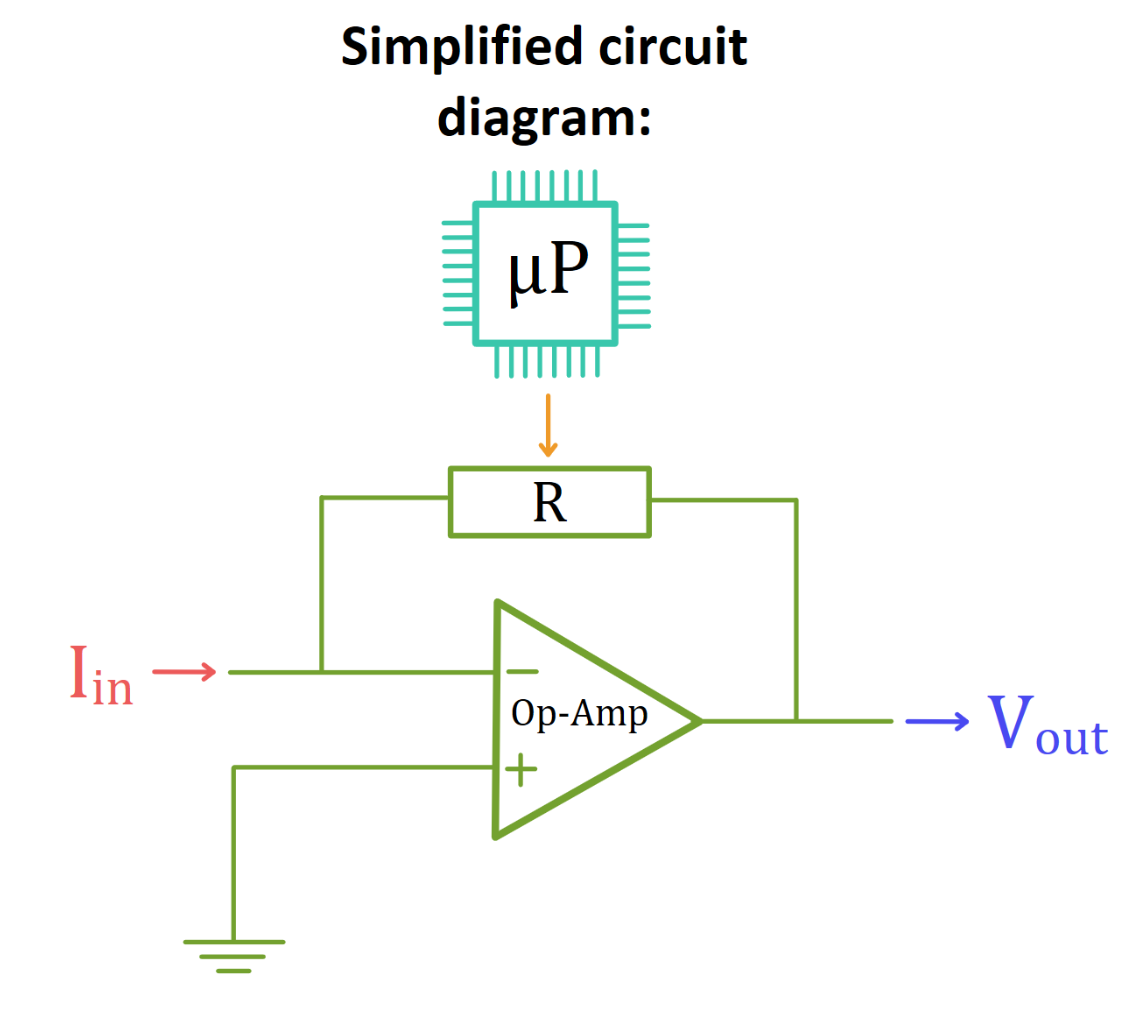
\includegraphics[width=0.8\linewidth]{Simplified_Circuit_Diagramv2.png}
    \caption{Simplified Circuit diagram of the switching TIA design}
    \label{fig:2}
\end{figure}

\subsection{Hardware topologies}

There are three TIA topologies that could be used for this design. This is a major consideration for the design, as the primary goal of the project is focused on the ability to change the gain of the TIA. \\

The first topology, in the top left corner of figure \ref{fig:3}, is the simplest and likely the most common. It puts feedback resistors in parallel with an op-amp, allowing switches to select which resistor, and therefore gain, is being used in the TIA circuit. NZMSL’s current TIAs use this topology with a manual dial physically switching out the resistors.
The other two topologies dedicate an individual op-amp for each level of gain. The benefit of this is it allows a specific op-amp with ideal characteristics to be selected for each gain value, instead of restricting the entire circuit to one op-amp which may behave optimally for some gain values, but not so for others. \\

The top right corner of figure \ref{fig:3} illustrates a series configuration of multiple op-amps. The first circuit would be the only transimpedance amplifier, all the rest would be regular non-inverting amplifiers as they no longer have to turn a current into a voltage, and would instead need to amplify the voltage from the last circuit to the next decade of gain. The switching in this case would only be on the output, and select which op-amps output to feed to the output of the system.  \\

\begin{figure}
    \centering
    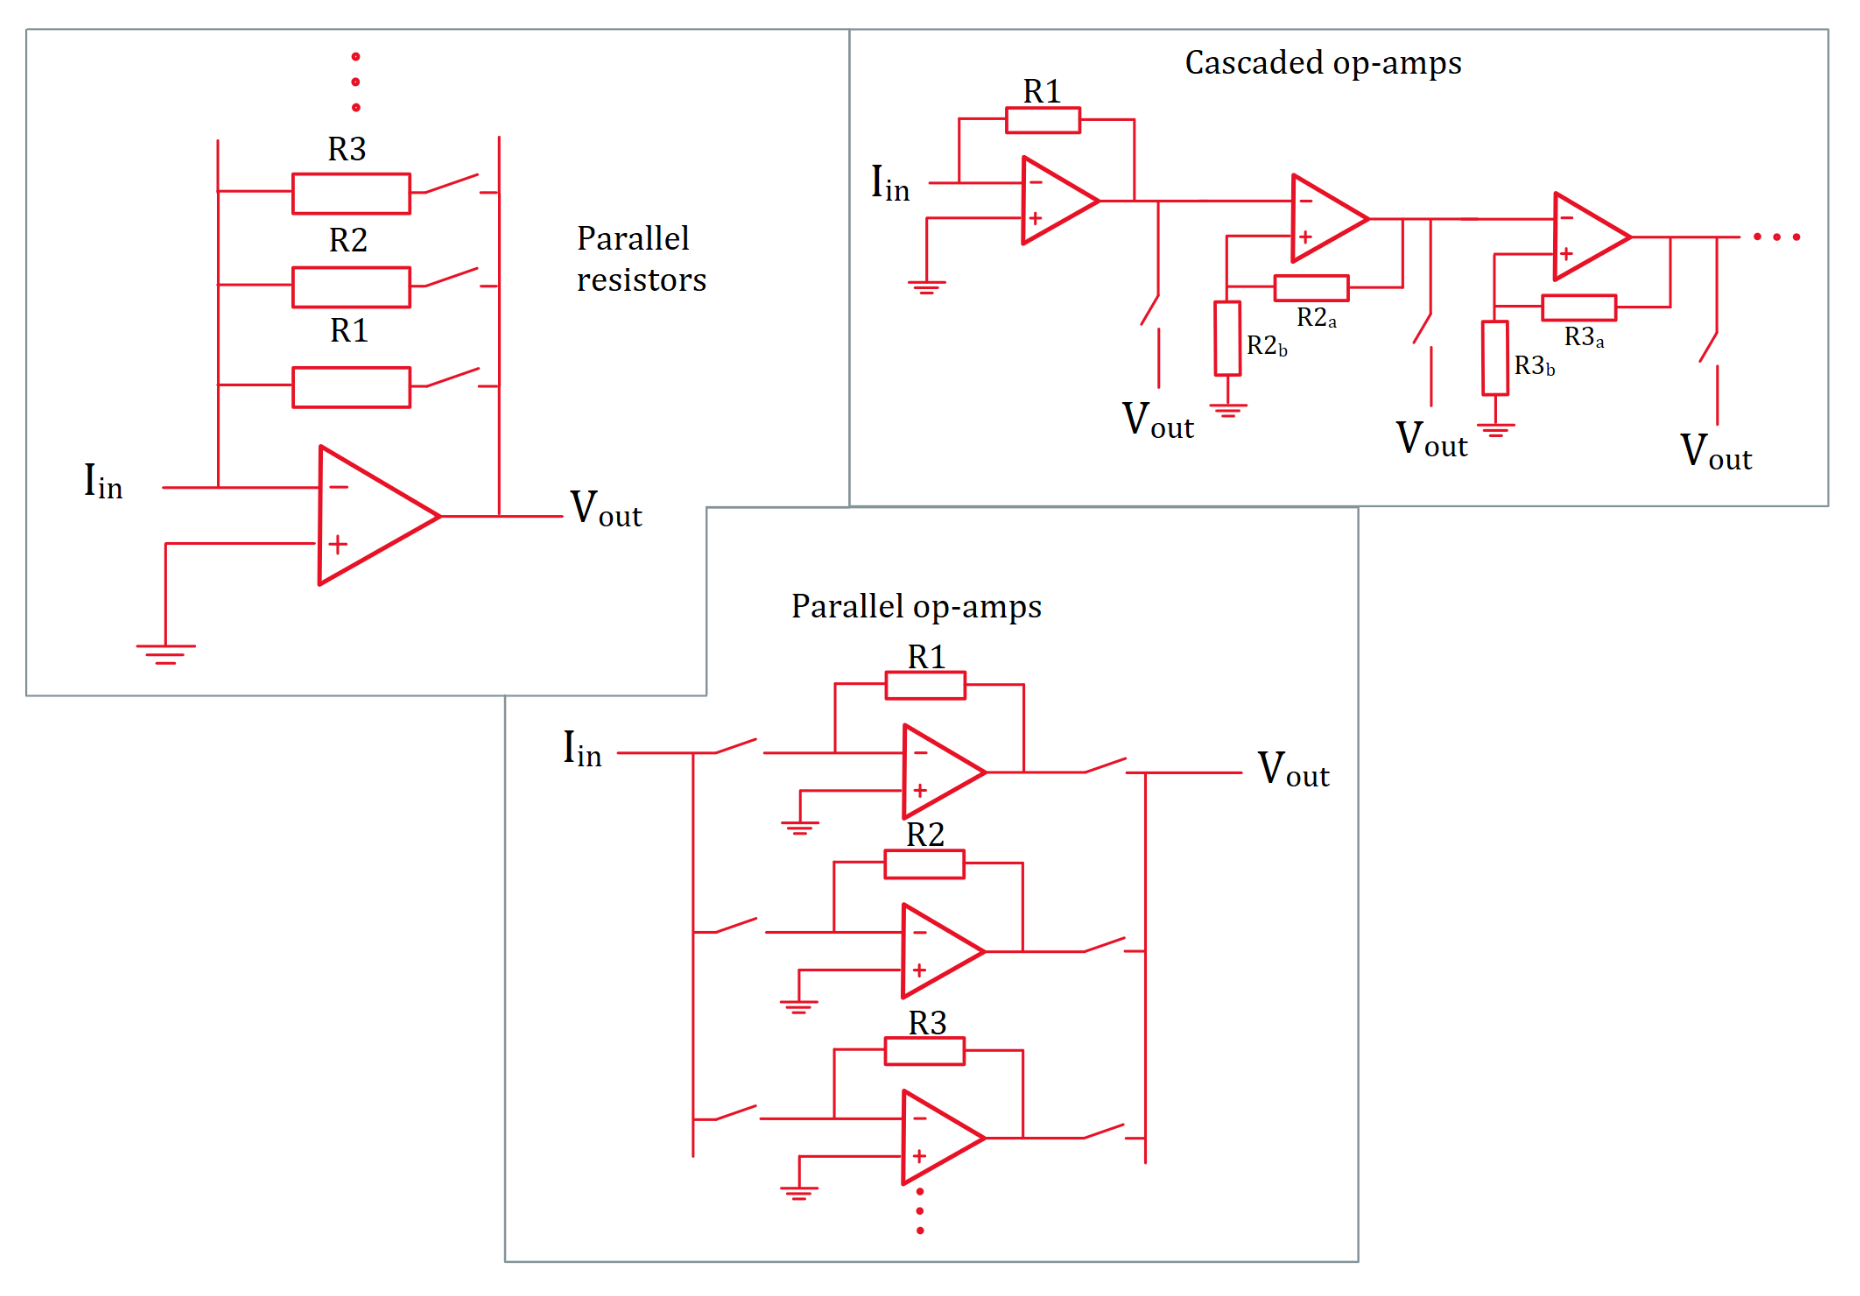
\includegraphics[width=0.8\linewidth]{TopologiesV3.png}
    \caption{Three possible TIA topologies.}
    \label{fig:3}
\end{figure}

The disadvantage of a set of TIA’s connected in series is that the first circuit will be a major limiting factor. If the first op-amp and feedback resistor receive a current that is beyond what they are designed to accurately amplify (whether it’s too low or high), it could distort the input and cascade that distortion all the way to the output, effectively nullifying the benefits of having multiple TIA circuits fine tuned to specific gain values. \\

The final design in figure \ref{fig:3} illustrates the chosen topology of this project. This design combines the benefits of both of the other topologies. It takes TIA circuits that have each been designed for a specific gain, and puts them in parallel to avoid unnecessarily modifying the input current, satisfying requirement R1.4. \\

\subsection{Switching considerations}

A factor which must be taken into account before implementation is that of leakage current across switches. Leakage currents across switches have the potential to tamper with the input current of the circuit, with a small portion being leaked through open switches into disconnected portions of the circuit. This has the potential to add error to both the input and output, even with switches being employed on both sides of the TIA. This would degrade the input signal, while the output signal could receive leakage current from one or more of the inactive areas of the circuit. The possibility of the output being tampered with is reduced as any leakage current would need to first pass the input side switch, pass through the TIA and then also leak through the output side switch.
To eliminate the possibility of any leakage currents, Latching relays were used for switching. Latching relays are electromechanical switches that maintain their state without any power needing to be applied. By way of being a mechanical contact switch reduces the chance of there being almost any leakage currents through latching relays. Because of the way latching relays work, the control current and the switched current are electrically isolated, meaning the control current will not interfere with the current being measured. Both of these characteristics make latching relays ideal for this application.\\

\textit{This whole section needs to be replaced with an explanation of how our switching works, and what it does to mitigate any issues} \\

\subsection{Software design}

\textit{Need a description of the software, and how it works}

\subsection{Power Supply}

As this is an active electronic design, it will need a power supply. Given that the output voltage needs to be able to reach 10V (as seen in requirement 2.1), the op-amps require at least 10V to power their rails. The BeagleBone however, needs 5V to be powered. The simplest solution is to power them separately with 12V and 5V power supplies. This is not the neatest or most user friendly approach, and could be replaced by using a single power supply with a DC-DC voltage converter in the system. However, neither neatness nor user-friendliness are high priorities in this design, therefore they are not necessary before end user implementation. \\

\section{Implementation}

\textit{The purpose of this section is for you to discuss how you transformed the technical solution (the design) to its realisation (the artifact). Similar to the Design section, you must provide clear and sufficient descriptions.} \\

\textit{Needs: a figure of the final schematic/PCB, and explanation of its layout. Also the final PCB in its case would be good}

\section{Evaluation}

\textit{The purpose of the evaluation section is to demonstrate whether you did or did not satisfy the project goals or specifications. If you can tie the performance of your design to some real specification then your evaluation is much stronger. “My code runs in 29 ms” is much weaker than “my code runs within the 30 ms window allowable for real-time performance of the. . . ”.} \\



\section{Conclusions \& Future Work}

\textit{Future work should not just be a list of things that you would have done if you had a little more time. Talk about new things that are possible now that you have finished your project. What projects could a ’489 student tackle next year if they started on their '489 project next year from your end point? HINT: This might be a possibility!} \\






% *** REFERENCES ***
\bibliographystyle{IEEEtran}
\bibliography{references}

\textit{Referencing and citation are important to avoid plagiarism. You must follow an appropriate citation format (e.g. IEEE, Chicago, APA, etc.)} \\



\end{document}
